\chapter{Implementação de um filtro de Kalman}\label{cap:kalman}

Os dados de visão são recebidos com ruído, que tem diversos causadores e é impossível de ser completamente eliminado. Tal ruído causa oscilação nas velocidades e derivadas superiores que são calculadas a partir das medidas de posição. Precisávamos de uma medida de velocidade mais confiável, então foi decidido que o ruido na posição seria tratado para diminuir seus efeitos no cálculo das velocidades do robô. Além disso, quando são usadas mais de uma câmera para filmar o jogo, cada câmera registra um determinado objeto numa posição ligeiramente distinta, demandando uma fusão sensorial.

O filtro de Kalman permite que a partir de uma medição ruidosa e um modelo dinâmico para o fenômeno sendo observado, seja obtida uma estimativa mais precisa do que a medição. Além disso, também pode ser utilizado para a fusão de diversas medidas resultando em uma estimativa mais precisa.

O filtro de Kalman é um estimador recursivo. Apenas o estado estimado do passo de tempo anterior e a medida atual são necessários para computar a estimativa para o estado atual. No que se segue, a notação $\displaystyle {\hat {\mathbf {x} }}_{n\mid m}$ representa a estimativa de ${\displaystyle \mathbf {x} }$ no tempo n dadas observação até o tempo $m \leq n$, inclusive.

O estado do filtro é representado por duas variáveis:

   ${\displaystyle {\hat {\mathbf {x} }}_{k\mid k}}$, a estimativa de estado a posteriori no tempo k dadas observações até o tempo k, inclusive;
   ${\displaystyle \mathbf {P} _{k\mid k}}$, a matriz de covariância do erro a posteriori (uma medida da acurácia estimada da estimativa do estado).

O filtro pode ser descrito em uma única equação, no entanto costuma ser conceitualizado em duas fases distintas: "Predição" e "Atualização". A fase de predição usa a estimativa de estado do passo anterior para produzir uma estimativa do estado no passo atual. Essa estimativa de estado predita também é conhecida como estimativa de estado a priori pois, embora seja uma estimativa do estado no passo atual, ela não inclui a informação da observação feita no passo atual. Na fase de atualização, a predição a priori atual é combinada a information da observação atual para refinar a estimativa de estado. Essa estimativa melhorada é chamada a estimativa de estado a posteriori.

Tipicamente, as duas fases se alternam, com a predição avançando o estado até a próxima observação agendada, e a atualização incorporando a observação. No entanto, isso não é necessário; se uma observação não está disponível por alguma razão, a atualização pode ser pulada e serem executados múltiplos passos de predição. Semelhantemente, se múltiplas observações independentes estão disponíveis ao mesmo tempo, múltiplos passos de atualização podem ser realizados (tipicamente com diferentes matrizes de observação $H_k$).

\section{Predição}
\begin{itemize}
  \item Estimativa de estado predita (a priori): ${\displaystyle {\hat {\mathbf {x} }}_{k\mid k-1}=\mathbf {F} _{k}{\hat {\mathbf {x} }}_{k-1\mid k-1}+\mathbf {B} _{k}\mathbf {u} _{k}}$
  \item Covariância estimada predita (a priori): ${\displaystyle \mathbf {P} _{k\mid k-1}=\mathbf {F} _{k}\mathbf {P} _{k-1\mid k-1}\mathbf {F} _{k}^{\mathrm {T} }+\mathbf {Q} _{k}}$
\end{itemize}

\section{Atualização}
\begin{itemize}
  \item Inovação ou resíduo pré-ajuste da medida: ${\displaystyle {\tilde {\mathbf {y} }}_{k}=\mathbf {z} _{k}-\mathbf {H} _{k}{\hat {\mathbf {x} }}_{k\mid k-1}}$
  \item Innovation (or pre-fit residual) covariance: ${\displaystyle \mathbf {S} _{k}=\mathbf {R} _{k}+\mathbf {H} _{k}\mathbf {P} _{k\mid k-1}\mathbf {H} _{k}^{\mathrm {T} }}$
  \item Ganho ótimo de Kalman: ${\displaystyle \mathbf {K} _{k}=\mathbf {P} _{k\mid k-1}\mathbf {H} _{k}^{\mathrm {T} }\mathbf {S} _{k}^{-1}}$
  \item Estimativa de estado atualizada (a posteriori): ${\displaystyle {\hat {\mathbf {x} }}_{k\mid k}={\hat {\mathbf {x} }}_{k\mid k-1}+\mathbf {K} _{k}{\tilde {\mathbf {y} }}_{k}}$
  \item Covariância estimada atualizada (a posteriori): ${\displaystyle \mathbf {P} _{k|k}=(\mathbf {I} -\mathbf {K} _{k}\mathbf {H} _{k})\mathbf {P} _{k|k-1}}$
  \item Resíduo da medida pós-ajuste: ${\displaystyle {\tilde {\mathbf {y} }}_{k\mid k}=\mathbf {z} _{k}-\mathbf {H} _{k}{\hat {\mathbf {x} }}_{k\mid k}}$
\end{itemize}

Após o estudo dos fundamentos do filtro de Kalman, foi implementada uma versão do filtro para ser executada junto do software de inteligência, construído em LabView.

Na Figura~\ref{fig:log_player} pode ser visto um detalhe do diagrama de blocos principal, mostrando o \textit{loop} que recebe os dados provenientes das câmeras e realiza a filtragem, através do bloco \textit{Detection Frame Estimator}.

\begin{figure}
	\centering
	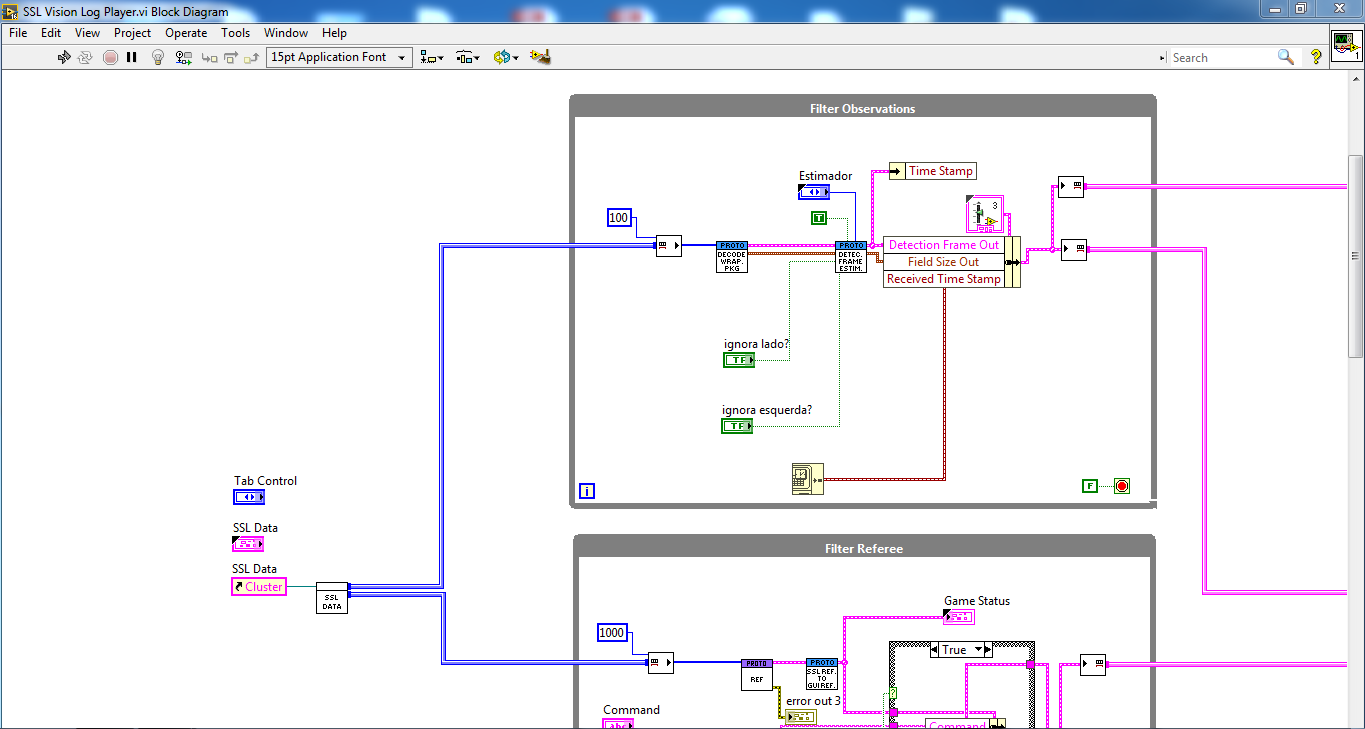
\includegraphics[scale=0.4]{SSL_Vision_Log_Player}
	\caption{Loop de filtragem dos dados da visão}
	\label{fig:log_player}
\end{figure}

Na Figura~\ref{fig:frame_estim} pode ser visto um detalhe do diagrama de blocos \textit{Detection Frame Estimator}, mostrando os blocos que tratam, separadamente, os dados das bolas, dos robôs do time aliado e do time adversário, usando blocos \textit{Kalman Balls Estimator} e \textit{Kalman Robots Estimator}.

\begin{figure}
	\centering
	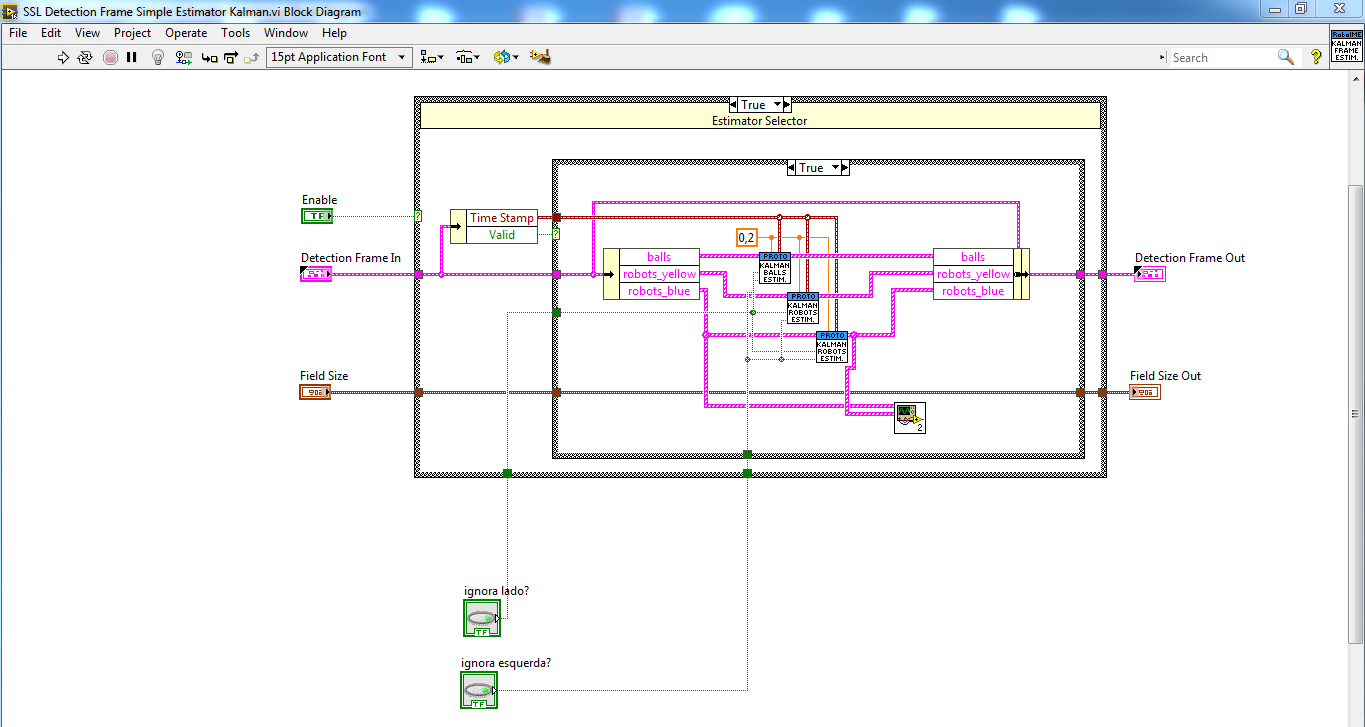
\includegraphics[scale=0.4]{Detection_Frame_Estimator}
	\caption{Detalhe do bloco Detection_Frame_Estimator}
	\label{fig:frame_estim}
\end{figure}

Na Figura~\ref{fig:kalman_balls} pode ser visto o bloco Kalman_Estimator_for_Balls, no qual as informações de posição das bolas são recebidas, é feita uma checagem do estado anterior do filtro, seguida por uma atualização do histórico de amostras e por fim, a filtragem propriamente dita. O bloco Kalman_Estimator_for_Robots é muito similar e não será mostrado. 

\begin{figure}
	\centering
	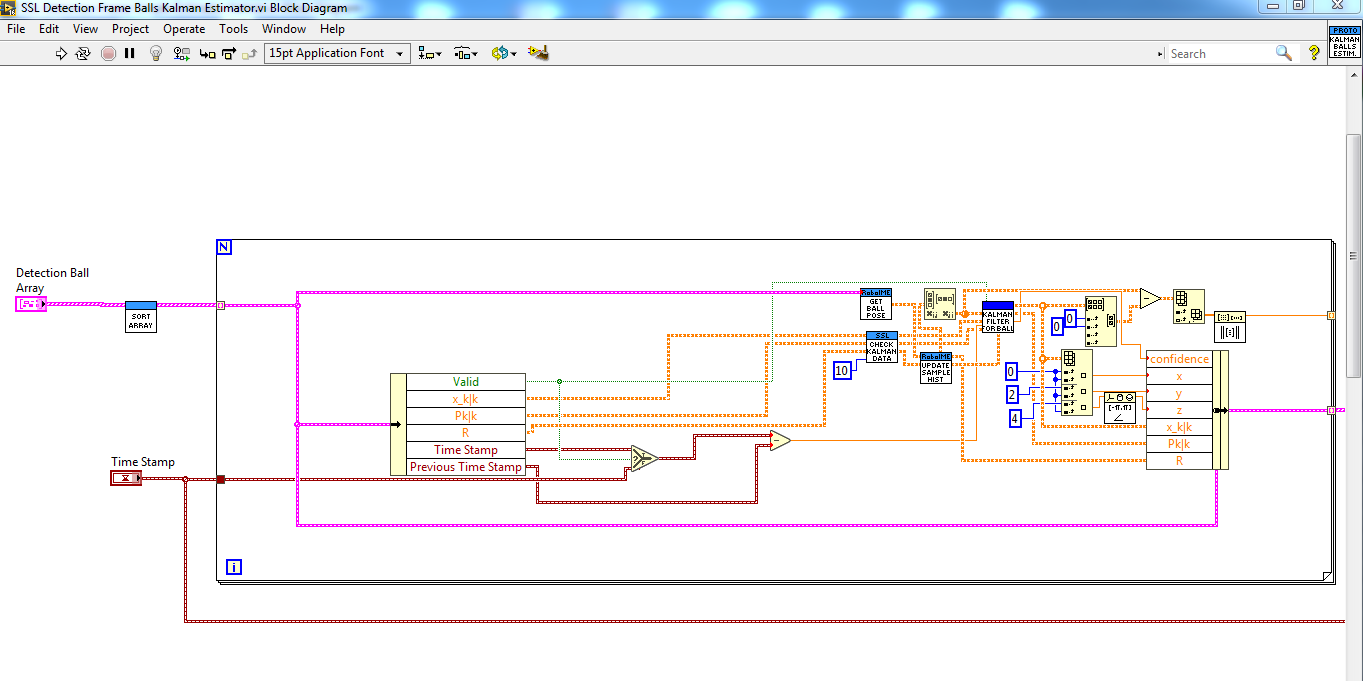
\includegraphics[scale=0.4]{Kalman_Estimator_for_Balls}
	\caption{Detalhe do bloco Kalman_Estimator_for_Balls}
	\label{fig:kalman_balls}
\end{figure}

%\begin{figure}
%	\centering
%	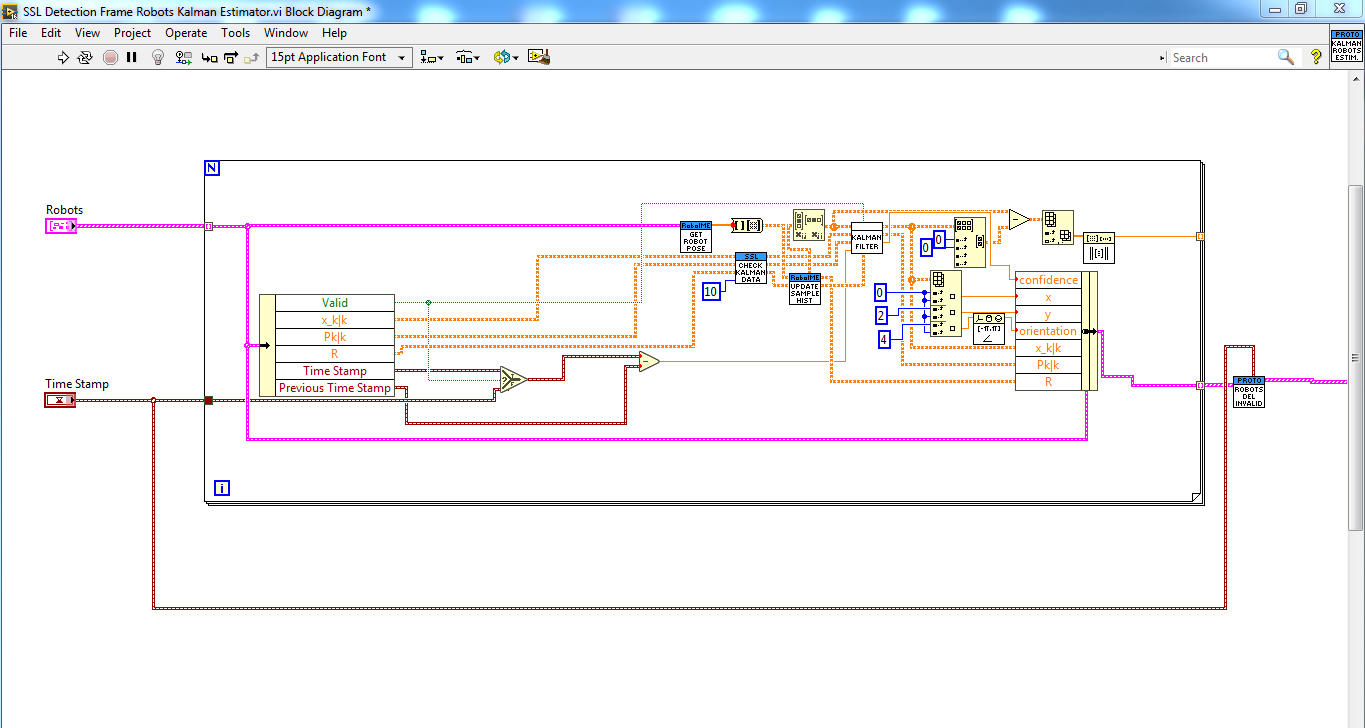
\includegraphics[scale=0.4]{Kalman_Estimator_for_Robots}
%	\caption{Detalhe do bloco Kalman_Estimator_for_Balls}
%	\label{fig:kalman_robots}
%\end{figure}

Na Figura~\ref{fig:kalman_balls_inside} pode ser vista a implementação de um filtro de Kalman propriamente dito, com os sinais de interesse indicados pelas suas equações de definição. O filtro para as posições dos robôs é muito similar, por isso não será mostrado.

\begin{figure}
	\centering
	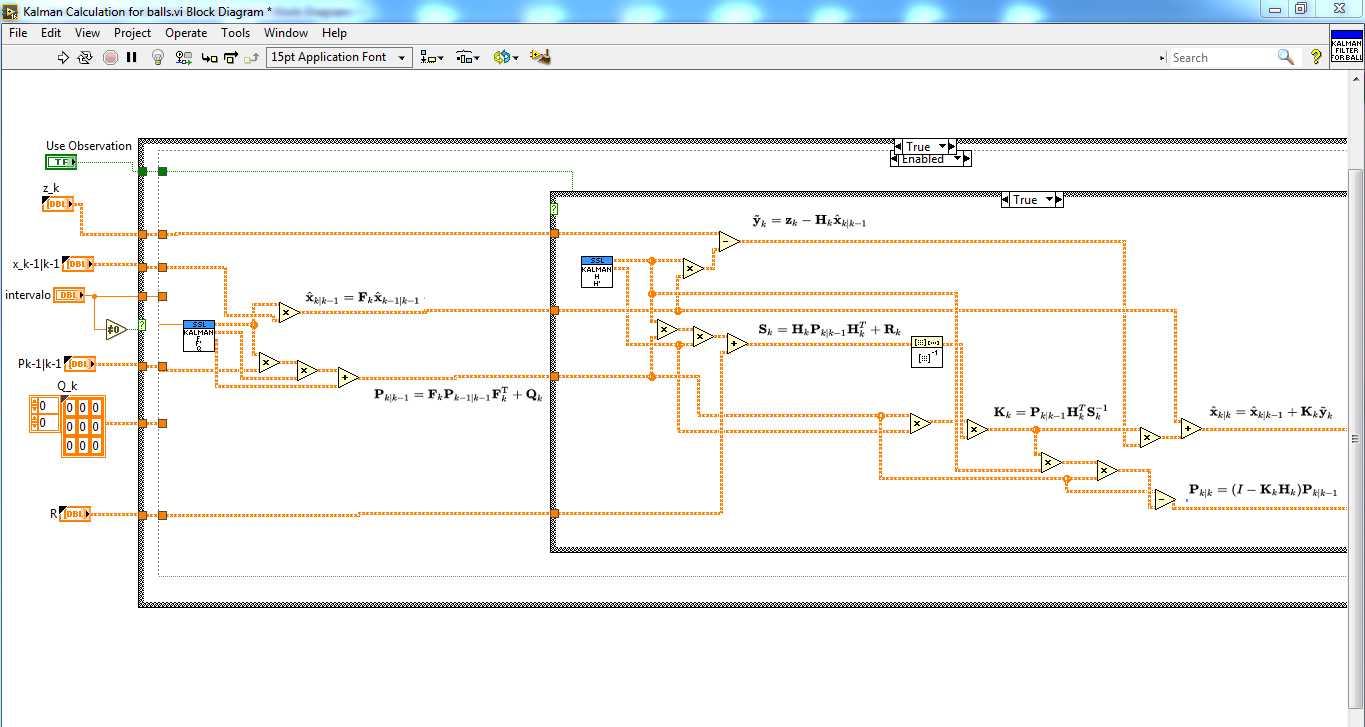
\includegraphics[scale=0.4]{Kalman_Filter_for_Balls_inside}
	\caption{Detalhe do bloco Kalman_Calculation_for_Balls}
	\label{fig:kalman_balls_inside}
\end{figure}

% Ramificação constante ou taxa constante

% vim: tw=80 et ts=2 sw=2 sts=2 ft=tex spelllang=pt_br,en

